\chapter{Application des techniques d'anonymisation dans le domaine agricole}
Jusqu'à présent, rares sont les études qui portent sur l'anonymisation des données dans le domaine agronomique.
Cela est en partie dû au fait que ces données sont en générale ouvertes et ne portent pas un caractère personnel. On peut facilement trouver,sur des plate-formes comme opendata ou datagouv, de grands volumes de données en rapport avec l'agro-environnement\cite{bouaziz_tome_nodate}. Cela est certes indispensable pour mener à bien des études comme par exemple le rapport entre le climat et l'apparition de certaines maladies des plantes, l'influences des pesticides sur l'environnement etc. 
Pour faire cela, on est souvent amené à croiser des données du type plantes cultivées, type de sol avec des données météorologiques localisées se rapportant à une parcelle de terrain. L'ensemble des parcelles cultivées en France étant répertoriées dans le \gls{RPG}, il apparaît clairement que croisé avec d'autres sources de données, le RPG peut permettre une ré-identification des agricultures, sources de données, d'où l'intérêt d'anonymiser également les données dans le domaine agronomique.


\subsection{Exemple de réidentification}
En parcourant un jeu de données sur le Plan régional de Modernisation des Bâtiments d’Élevage "classique" en Auvergne (PMBE)- Attributions 2013/2015  de la plateforme opendata, j'ai pu isoler un enregistrement \ref{fig:Enregistrement d'une base de données publique}
\begin{figure}
    \centering
    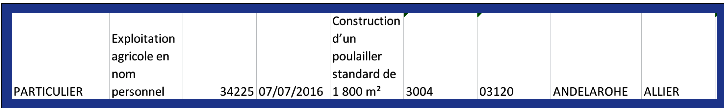
\includegraphics[width=\textwidth]{images/anonymisation/exemple1_anonymisation.png}
    \caption{Enregistrement dans base de données publique}
    \label{fig:Enregistrement d'une base de données publique}
\end{figure}
Après quelques recherches sur un moteur de recherche, en utilisant les mots clés poulailler, Allier, 1800\begin{math}m^{2}\end{math} j'ai trouvé deux articles de journal qui en parlent et à partir de là j'ai pu identifier la personne propriétaire du poulailler.
\begin {figure}
\begin{center}
    \hbox{ 
    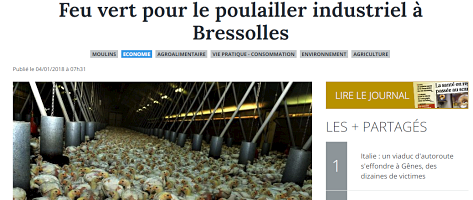
\includegraphics[height=3cm]{images/anonymisation/exemple2_anonymisation.png}
    \hspace*{1cm}  %% pour mettre un espace (horizontal) de 5cm entre les deux images
    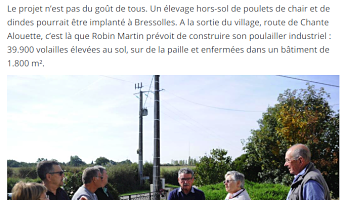
\includegraphics[height=3cm]{images/anonymisation/exemple3_anonymisation.png}
  }
\caption{Articles de Journal}
\label{fig : Articles de Journal}
\end{center}
\end {figure}

Dans l'exemple précèdent, on remarque à quel point il peut être parfois facile de ré-identifier une personne à partir de données publiques. Dans la suite de ce rapport, j'essaye de transposer  les techniques d'anonymisation vues précédemment sur des données à caractère agronomique en se focalisant surtout sur la dimension spatiale des données car la dimension temporelle peut être facilement masquée. Le but étant de conserver l'utilité des données.

%%%%%%%%%%% GÉNÉRALISATION %%%%%%%%%%%
\section{La Généralisation}
L'approche la plus couramment utilisée pour rendre anonyme des données géographique est la généralisation. Elle se rapporte à la technique de généralisation vue plus haut. Elle consiste à réduire la précision au niveau géographiques. On crée ainsi de classe d’équivalence, avec des enregistrements ayant une localisation spatiale identique. Selon la clarté sur les données et le niveau de sécurité que l’on souhaite, la réduction de la précision géographique peut être utilisée pour contrôler la taille des classes d’équivalence. Deux techniques ressortent parmi les techniques de généralisation:  
\begin{itemize}
    \item Le Changement d’échelle : cette approche consiste à réduire la précision géographique en élargissant les zones visées par les attributs géographiques. Le changement d'échelle peut s'obtenir de plusieurs façons : \begin{itemize}
        \item  On peut supprimer les trois derniers chiffres des codes postaux, se référent à une grande zone géographique.
        \item   Les coordonnées GPS peuvent être remplacées par le nom de la commune, de la région ou du canton.
    \end{itemize} 
    Le changement d’échelle est donc tout simplement une application du k-anonymat sur des données géographiques. 
    \item   Le Carroyage : Le carroyage est une technique de quadrillage utilisée en topographie, afin de rassembler et de traiter des données en vue d’une exploitation cartographique ou statistique. Il est très similaire au changement d’échelle à mise à part que pour cette techniques, toutes les subdivisions sont de même taille.
\end{itemize}

%%%%%%%%%%% Génération des données %%%%%%%%%%%
\section{La Génération des données}
Une autre approche serait la génération des données. C'est-à-dire qu'a partir d'un certain jeu de données, on pourrait en générer un autre en ajoutant ou en supprimant de l'information. Cela reviendrait à appliquer la technique de l'ajout de bruit.Il resterait alors à surmonter la difficulté de rendre cohérent les données ainsi générées. En effet, comme vu précédemment, l'ajout de bruit est souvent confronté à deux problèmes : soit le bruit n'est pas suffisant et dans ce cas l'anonymisation n'est pas efficace, soit il y a beaucoup de bruit et la donnée perd son utilité.
%%%%%%%%%%% Déplacement des Coordonnées %%%%%%%%%%%
\section{Déplacement des coordonnées}
 La dernière approche qui peut être utilisée sur des coordonnées spatiales consisterait à faire une permutation(brouillage) des coordonnées. Il faudra cependant respecter certaines contraintes pour garder la cohérence des données ainsi que leur utilité. Exemples : 
 \begin{itemize}
     \item deux points de coordonnées proches avant le brouillage, doivent l'être aussi après le brouillage
     \item brouiller les coordonnées de façon uniforme dans chaque zone comme dans la Figure \ref{fig:Brouillage uniforme}
     \item Mais si par exemple la station météo la plus proche d’une parcelle de la zone A se trouve dans la zone B, alors brouiller les coordonnées en tenant compte du voisinage. Figure \ref{fig:Brouillage avec gestion de voisinage}
 \end{itemize}
 
 \begin{figure}[!h]
    \centering
    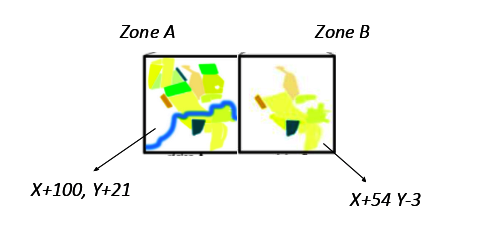
\includegraphics[width=.5\textwidth]{images/anonymisation/brouillage_image1.png}
    \caption{ Brouillage uniforme}
    \label{fig:Brouillage uniforme}
\end{figure}
\begin{figure}[!h]
    \centering
    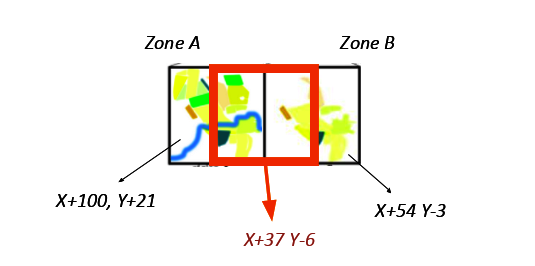
\includegraphics[width=.5\textwidth]{images/anonymisation/brouillage_image2.png}
    \caption{ Brouillage avec gestion de voisinage}
    \label{fig:Brouillage avec gestion de voisinage}
\end{figure}
